%!TEX encoding = UTF8
%!TEX root =notes.tex

\chapter{Signes, variations, et extrema}

Le but de ce chapitre est de traiter la partie \og Étudier les variations et les extremums d'une fonction \fg~du bulletin officiel.

Le contenu du chapitre est le suivant.
	\begin{itemize}
		\item Résoudre une équation, une inéquation produit ou quotient, à l'aide d'un tableau de signes.
		\item Croissance, décroissance, monotonie d'une fonction définie sur un intervalle. Tableau de variations.
		\item Maximum, minimum d'une fonction sur un intervalle.
		\item Pour une fonction affine, interprétation du coefficient directeur comme taux d'accroissement, variations selon le signe.
	\end{itemize}

Les capacités attendues sont les suivantes.
	\begin{itemize}
		\item Relier représentation graphique et tableau de variations.
		\item Déterminer graphiquement les extrema d'une fonction sur un intervalle.
		\item Exploiter un logiciel de géométrie dynamique ou de calcul formel, la calculatrice ou Python pour décrire les variations d'une fonction donnée par une formule.
		\item Relier sens de variation, signe, et droite représentative d'une fonction affine.
	\end{itemize}
	

Les manipulations d'inégalités ont été étudiées dans la section \ref{subsec:ineg} du chapitre \ref{chap:3}.

\section{Domaine de définition, signes, tableaux de signes}

\subsection{Domaine de définition}

\dfn{Domaine de définition, valeurs interdites}{
	Soit $f$ une fonction quelconque. On souhaite connaître le domaine le plus grand possible sur lequel définir $f$.
	On l'appelle le \emph{domaine de définition}, qu'on note $\D_f$.
	
	Pour cela, on étudie la fonction sur $\R$ dont on supprime les \emph{valeurs interdites}, c'est-à-dire les antécédents pour lesquels $f$ est mal définie.
	On étudiera dans ce chapitre deux conditions qui permettront d'identifier ces valeurs interdites :
		\begin{enumerate}
			\item l'expression sous une racine carrée doit toujours être positive ou nulle ; et
			\item un dénominateur ne doit jamais être nul.
		\end{enumerate}
}{}

\ex{Valeurs interdites}{
	Soit $f$ la fonction donnée par
		\[ f(x) = \dfrac{\sqrt{7-2x}}{x}. \]
	On identifie deux conditions qui doivent être vérifées pour que calculer $f(x)$ ait un sens :
		\begin{enumerate}
			\item $7-2x \geq 0$ ; et
			\item $x \neq 0$.
		\end{enumerate}
	La première inégalité nous impose que $x \leq \dfrac72$, et la deuxième condition supprime $0$.
	On obtient donc
		\[ \D_f = \left] \minfty; \frac72 \right] - \{0\} =  \left] \minfty; 0 \right[ \cup  \left] 0; \frac72 \right]. \]
}{}

\subsection{Étude de signes : tableaux de signes}

\dfn{Signe d'un nombre réel}{
	Soit $x\in\R$ un nombre réel quelconque.
	On dit que
		\begin{itemize}
			\item $x$ est \emph{strictement positif} si $x>0$ ;
			\item $x$ est \emph{strictement négatif} si $x<0$ ;
			\item $x$ est \emph{nul} si $x=0$.
		\end{itemize}
	En français, dire \og $x$ est positif \fg~signifie que $x$ est positif ou nul ($x\geq0$).
	Il est préférable de dire \emph{positif ou nul} pour éviter toute ambiguïté.
}{}

\nt{
	Pour simplifier la notation, au lieu d'écrire \og $A >0$ et $B > 0$ \fg, on écrira juste \og$A, B > 0$\fg.
}{}

\thm{Signe du produit}{
	Soit $A, B \in \R$ deux réels.
	On distingue trois cas sur le signe du produit $A \cdot B$.
		\begin{enumerate}
			\item Si $A \cdot B = 0$, alors $A=0$ ou $B=0$. (le \og ou \fg~est inclusif)
			\item Si $A \cdot B > 0$, alors $A$ et $B$ ont le même signe :
				\begin{enumerate}[label=\roman*)]
					\item soit $A, B > 0$ ;
					\item soit $A, B < 0$.
				\end{enumerate}
			\item Si $A \cdot B < 0$, alors $A$ et $B$ sont de signes opposés :
				\begin{enumerate}[label=\roman*)]
					\item soit $A> 0$ et $B < 0$ ;
					\item  soit $A < 0$ et $B > 0$.
				\end{enumerate}
		\end{enumerate}
}{thm:signe-produit}


\cor{Signe du quotient}{
	Soit $A, B \in \R$ deux réels. On suppose que $B \neq 0$.
	
	Alors, le signe de $\dfrac1B$ est le même que celui de $B$, et donc le signe du quotient
		\[ \dfrac{A}{B} = A \cdot \dfrac1B \]
	suit les mêmes règles que celui du produit $A \cdot B$.
}{}

\ex{Problème de signe}{
	On souhaite connaître pour quels $x\in\D$ l'inégalité suivante est vérifée.
		\[ f(x) = \dfrac{6x^2 - 5x - 4}{3-x} \geq 0. \]
	En premier lieu, remarquons que certaines valeurs sont interdites : ce sont les valeurs pour lesquelles le dénominateur s'annule.
	Le domaine de $f$ est donc tout $\R$ perforé en $x=3$ :
		\[ \D = \R - \{3 \} = ]\minfty ; 3[ \cup ]3 ; \pinfty[. \]
	
	Ensuite, on vérifie qu'on a bien 
		\[ (3x-4)(2x+1) = 6x^2 - 5x - 4, \]
	factorisation qui nous est donnée par le professeur.
	
	On obtient alors
		\[ f(x) = \dfrac{(3x-4)(2x+1)}{3-x}, \]
	et connaître le signe de chacun des facteurs permettra de connaitre le signe de $f$.
	
	On a les équivalences suivantes.
		\begin{align*}
%			3x-4 \geq 0 && \iff && x \geq \dfrac43, \\
%			2x+1 \geq 0 && \iff && x \geq -\dfrac12, \\
%			3-x \geq 0 && \iff && x \leq 3
			3x-4 \geq 0 && 2x+1  \geq 0 && 3-x \geq 0 \\
			\iff\quad && \iff\quad && \iff\quad \\
			x \geq \dfrac43 && x \geq -\dfrac12 && x \leq 3
		\end{align*}
	On synthétise les signes obtenus dans le tableau suivant qu'on appelle \emph{tableau de signes}.
	\begin{tikzpicture}
		\tkzTabInit
		 %[lgt=3,espcl=1.5]
	       		{$x$ / 1 , $3x-4$ / 1, $2x+1$ / 1, $3-x$ / 1, $f(x)$ / 1}
	       		{$\minfty$, $-\dfrac12$, $\dfrac43$, $3$, $\pinfty$}
	       		
		\tkzTabLine
			{,-,t,-,z,+,t,+}
		\tkzTabLine
			{,-,z,+,t,+,t,+}
		\tkzTabLine
			{,+,t,+,t,+,z,-}
		\tkzTabLine
			{,+,t,-,t,+,d,-}
	\end{tikzpicture}
	
	Le signe de $f(x)$ dans la première case est déduit du fait qu'on fait \og moins $\times$ moins $\times$ plus \fg, qui donne \og plus \fg, car le produit d'un positif avec deux négatifs est positif. On fait idem pour le reste.
	
	De plus, on note avec les doubles barres $||$ la valeur interdite $x=3$.
	
	En conclusion, l'ensemble des $x \in \D$ vérifiant $f(x) \geq 0$ est donné par
		\[ \left\{ x \in \R-\{3\} \text{ tq. } f(x) \geq 0 \right\} = \left]\minfty ; -\dfrac12 \right] \bigcup \left[ \dfrac43 ; 3 \right[. \]
}{}


\ex{Problème de racines}{
	On souhaite connaître les solutions de l'équation du deuxième degré d'inconnue $x\in\R$ :
		\[ 21 x^2 - 11 x - 2  = 0. \]
	Ce problème est un large domaine d'étude en mathématiques, c'est le problème des \emph{racines} d'une fonction. Ici, la fonction est $f(x) = 21 x^2 - 11 x - 2 $, et ses racines sont les antécédents qui annulent $f$.
	
	Plusieurs stratégies s'offrent à nous pour résoudre $f(x)=0$ : 
		\begin{itemize}
			\item Tracer $\C_f$ et lire les racines graphiquement. Cette méthode est utile pour approximer, mais ne permet pas d'obtenir les solutions exactes (ni le nombre de solutions, d'ailleurs).
			\item Tester des valeurs à partir du tracé. On pourrait démarrer vers une valeur approximative lue graphiquement puis se diriger vers la racine en affinant le pas au fur et à mesure. Cette méthode est très utilisée en pratique (\emph{cf.} la  dichotomie au chapitre d'algorithmique) mais ne permet parfois pas non plus d'obtenir une solution exacte.
			\item Essayer de factoriser $f(x)$ en un produit de deux expressions linéaire et utiliser le théorème \ref{thm:signe-produit}. L'avantage est qu'on obtient des solutions exactes. Un (gros) inconvénient est que cela n'est pas faisable pour toutes les fonctions $f$ (voir le théorème d'Abel-Ruffini). Pour les fonctions du deuxième degré, ça fonctionne cependant tout le temps : la résolution générale est au programme de $1$ère.
		\end{itemize}
	
	Ici, on vérifie que
		\begin{align*}
			(3x-2)(7x+1) &= 3x(7x + 1) - 2(7x+1) \\
							&= 21x^2 + 3x - 14x - 2 \\
							&= 21x^2 - 11x - 2 \\
							&= f(x).
		\end{align*}
	D'après le théorème  \ref{thm:signe-produit}, on a
		\begin{align*}
			&& f(x) = 0  && \\
			&& (3x-2)(7x+1) = 0 && \\
			3x-2 = 0 && \text{ ou }&& 7x + 1 = 0 \\
			x = \dfrac23 && \text{ ou } && x = -\dfrac17
		\end{align*}
}{}

\section{Variations et tableaux de variations}

\subsection{Définitions}

\dfn{Variations}{
	Soit $f : \D \rightarrow \R$ une fonction $f$ quelconque sur un intervalle $I\subseteq\R$.
	Alors
		\begin{itemize}
			\item On dit que $f$ est \emph{croissante} si, pour tous les $x,y\in I$ du domaine,
				\begin{align*}
					x < y && \implies && f(x) \leq f(y).
				\end{align*}	
			On interprète l'implication ainsi :
			\begin{center}
				\og lorsqu'on augmente l'abscisse $x$, l'ordonnée $f(x)$ augmente \fg.
			\end{center}
				
			\item On dit que $f$ est \emph{décroissante} si, pour tous les $x,y\in I$ du domaine,
				\begin{align*}
					x < y && \implies && f(x) \geq f(y).
				\end{align*}
			On interprète l'implication ainsi :
			\begin{center}
				\og lorsqu'on augmente l'abscisse $x$, l'ordonnée $f(x)$ diminue \fg.
			\end{center}
				
			\item On dit que $f$ est \emph{constante} si, pour tous les $x\in I$ du domaine, et pour une certaine constante $K\in\R$,
				\begin{align*}
					f(x) = K.
				\end{align*}
		\end{itemize}
	On définiera de la même façon \og strictement croissante \fg ~ (respectivement décroissante) en remplaçant l'inégalité large $\leq$ (resp. $\geq$) par l'inégalité stricte $<$ (resp. $>$).
}{}

\ex{Variation d'une fonction affine}{
	On considère $f(x) = -3x + 8$, une fonction affine sur $\R$.
	Comme $\C_f$ est une droite, on s'attend à ce que $f$ soit soit croissante, soit décroissante, soit constante.
	
	Prenons donc $x<y$ deux nombres réels quelconques.
	Comme $f$ n'est clairement pas constante, on essaye d'obtenir soit $f(x) < f(y)$, soit $f(y) < f(x)$.
	
	Le coefficient directeur $-3$ étant négatif, il change le sens de l'inégalité lorsqu'on multiplie par celui-ci.
	\begin{align*}
		x &< y \\
		-3x &> -3y \\
		-3x + 8 &> -3y + 8  \\
		f(x) &> f(y)
	\end{align*}
	On lit ce qu'on a obtenu ainsi : si on prend deux antécédents $x, y$ avec $x$ à gauche de $y$, alors $f(x)$ est au-dessus de $f(y)$.
	Graphiquement, la droite $\C_f$ doit nécessairement descendre pour aller de $(x, f(x))$ à $(y, f(y))$.
	Par définition, $f$ est décroissante. 
	
	On synthétise les variations obtenues dans le tableau suivant qu'on appelle \emph{tableau de variations}.
	
	\begin{center}
	\begin{tikzpicture}
		\tkzTabInit
		 %[lgt=3,espcl=1.5]
	       		{$x$ / 1 , $f(x)$ / 2}
	       		{$\minfty$,,, $\pinfty$}
	       		
		\tkzTabVar
			{+/, R/, R/, -/}
	\end{tikzpicture}
	\end{center}
	
	Le tableau n'est pas très intéressant pour l'instant car les variations des fonctions affines ne le sont pas particulièrement...
}{}

\subsection{Cas particulier : fonctions affines}

\thm{Variation d'une fonction affine}{
	Soit $f$ une fonction affine où $a, b \in\R$ sont ses deux paramètres réels.
		\begin{align*}
			f(x) = a x + b && (x\in\R)
		\end{align*}
	On distingue trois cas de figure.
		\begin{itemize}
			\item Si $a < 0$, alors $f$ est strictement décroissante.
			\item Si $a=0$, alors $f$ est constante.
			\item Si $a>0$, alors $f$ est strictement croissante.
		\end{itemize}
}{thm:affine-var}
%%%%%%%% MAYBE SKIP THIS? 
%%%%%%%% je pense que dy/dx est plus clair : si x monte et y descend, ça fait negatif/positif = négatif, pex.
%%%%%%%% après faut qu'ils soient convaincus de a=dy/dx et personne n'a réussi à le démontrer dans le bonus :((
%\pf{Démonstration du théorème \ref{thm:affine-var}}{
%	Si $a=0$, $f$ est clairement constante car
%		\begin{align*}
%			f(x) = b \qquad \text{ pour tout $x\in\R$}.
%		\end{align*}
%	
%	Sinon, on utilise les règles de manipulation des inégalités du théorème \ref{thm:ineg} vues au chapitre \ref{chap:3}.
%	
%	Si $a>0$, alors, pour tous les $x,y \in \R$ tels que $x < y$, on a
%		\begin{align*}
%			x &< y \\
%			a \cdot x &< a \cdot y \\
%			a \cdot x + b &< a \cdot y + b \\
%			f(x) &< f(y),
%		\end{align*}
%	et $f$ est donc strictement croissante.
%	
%	Si $a<0$, alors, pour tous les $x,y \in \R$ tels que $x < y$, on a
%		\begin{align*}
%			x &< y \\
%			a \cdot x &> a \cdot y \\
%			a \cdot x + b &> a \cdot y + b \\
%			f(x) &> f(y),
%		\end{align*}
%	et $f$ est donc strictement décroissante.
%}{}
\pf{Démonstration du théorème \ref{thm:affine-var}}{
	Soient $(x_A;y_A), (x_B; y_B) \in \C_f$ deux points distincts de la droite $\C_f$.
	Supposons de sucroît que $x_A < x_B$, c'est-à-dire que $A$ soit à gauche de $B$ dans le plan.
	
	Le dénominateur du coefficient directeur
		\[ a = \dfrac{y_B - y_A}{x_B-x_A} \]
	 est positif, et donc le numérateur détermine son signe.
	 
	 Si $a<0$, c'est que $y_B < y_A$, et donc que la fonction $f$ est décroissante.
	 Graphiquement, le point $A$ est à gauche et au-dessus du point $B$, et la droite descend.
	 
	 Les autres cas sont similaires.
}{}

\ex{Variation et signe d'une fonction affine}{
	On considère $f(x) = \dfrac25x + 12$, une fonction affine sur $\R$.
	Comme le coefficient directeur est $\dfrac25 > 0$, $f$ est croissante.
	Par conséquent, on peut connaître son signe en connaissant là où elle s'annule (son unique racine existe tant que $f$ n'est pas constante).
	
	On trouve $f(-30) = 0$, et on synthétise les résultats dans le tableau suivant.
	
	\begin{center}
	\begin{tikzpicture}
		\tkzTabInit
		 %[lgt=3,espcl=1.5]
	       		{$x$ / 1 , Variation de $f(x)$ / 2, Signe de $f(x)$ / 1}
	       		{$\minfty$,, $-30$,, $\pinfty$}
	       		
		\tkzTabVar
			{-/,  R/, R/, R/, +/}
		\tkzTabIma
			{1}{5}{3}{0}
			
		\tkzTabLine
			{,,-,,z,,+}
	\end{tikzpicture}
	\end{center}
	
	Le signe est déduit des variations de $f$ : comme $f$ est croissante et qu'elle s'annule en $-30$, son signe est nécessairement négatif avant et positif après.
}{}

\begin{figure}[h!]
	\begin{subfigure}{0.33\textwidth}
	\centering
	\begin{tikzpicture}[>=stealth, scale=.7]
	\begin{axis}[xmin = -1, xmax=1, ymin=-2, ymax=2, axis x line=middle, axis y line=middle, axis line style=<->, xlabel={}, ylabel={},ticks = none, grid=none]
	
		\addplot[very thick, myb, domain = -1:1] {2*x-.7} node[pos=.8, above=3pt] {\Large $\C_f$};
		\draw (axis cs: -.5, 1.5) node {\Huge \underline{$a>0$}};
	\end{axis}
	\end{tikzpicture}
	\caption{$f$ est croissante.}
	\end{subfigure}
	%\hspace{2cm}
	\begin{subfigure}{0.33\textwidth}
	\centering
	\begin{tikzpicture}[>=stealth, scale=.7]
	\begin{axis}[xmin = -1, xmax=1, ymin=-2, ymax=2, axis x line=middle, axis y line=middle, axis line style=<->, xlabel={}, ylabel={},ticks = none, grid=none]
	
		\addplot[very thick, myb, domain = -1:1] {-1.5*x-.5} node[pos=.4, below=3pt] {\Large $\C_f$};
		\draw (axis cs: -.5, 1.5) node {\Huge \underline{$a<0$}};
	\end{axis}
	\end{tikzpicture}
	\caption{$f$ est décroissante.}
	\end{subfigure}
	\begin{subfigure}{0.33\textwidth}
	\centering
	\begin{tikzpicture}[>=stealth, scale=.7]
	\begin{axis}[xmin = -1, xmax=1, ymin=-2, ymax=2, axis x line=middle, axis y line=middle, axis line style=<->, xlabel={}, ylabel={},ticks = none, grid=none]
	
		\addplot[very thick, myb, domain = -1:1] {-.6} node[pos=.7, below] {\Large $\C_f$};
		\draw (axis cs: -.5, 1.5) node {\Huge \underline{$a=0$}};
	\end{axis}
	\end{tikzpicture}
	\caption{$f$ est constante.}
	\end{subfigure}
	\caption{Courbes représentatives de fonctions affines $f(x) = ax+b$ selon le signe du coefficient directeur $a$.}
\end{figure}

\subsection{Fonctions parentes : impact sur les variations}

À partir des variations d'une fonction qu'on connaît bien (par exemple une fonction affine, la fonction carré, et on en verra d'autres au chapitre Fonctions de référence), on peut déduire les variations de toute une famille de fonctions apparentées.

On distingue trois types de fonctions parentes à partir d'une courbe représentative : on considère son translaté (horizontalement et verticalement séparément) et son homothétie (agrandissement, réduction, et même symétrie).

\ex{ajout d'une constante}{
	Considérons $f$ une fonction quelconque sur $\R$ et $g$ définie par
		\[ g(x) = f(x)+1. \]
	Pour calculer $g(0)$, on utilise donc la définition $g(0) = f(0) + 1$.
	De façon identique, $g(-3) = f(-3) + 1$, $g(12) = f(12) + 1$, etc…
	
	D'un point $(x; f(x))$ de la courbe $\C_f$, on peut donc en déduire le point $(x ; g(x)) = (x ; f(x)+1) = (x ; f(x)) + \pvec{0}{1}$ de la courbe $\C_g$.
	Graphiquement, la courbe $\C_f$ est translatée de $1$ unité vers le haut pour obtenir $\C_g$
	
	Pour $h(x) = f(x) - 2$, on obtient les graphes suivants.
	\begin{center}
	\begin{tikzpicture}[scale=1]
		\begin{axis}[xmin = -10, xmax=10, ymin=-4.25, ymax=4.25, axis x line=middle, axis y line=middle, axis line style=->, grid=both,
		%ytick={-4,-3,...,2,3}, xtick={-11, -10,...,-4,-3},
	    	%every y tick label/.style={
	        %anchor=near yticklabel opposite,
	        %xshift=0.2em,
	    	%}
	    	]
		% g cos
		\addplot[no marks, myb, -, very thick] expression[domain=-10:10, samples=50]{.01*(x+6)*(x+3)*(x-5)}
		node[pos=.5, below]{$\mathcal{C}_f$};
		\addplot[no marks, myr, -, very thick] expression[domain=-10:10, samples=50]{.01*(x+6)*(x+3)*(x-5)+1}
		node[pos=.2, above]{$\mathcal{C}_g$};
		\addplot[no marks, myg, -, very thick] expression[domain=-10:10, samples=50]{.01*(x+6)*(x+3)*(x-5)-2}
		node[pos=.5,below]{$\mathcal{C}_h$};
		\end{axis}
	\end{tikzpicture}
	\end{center}
}{}

\ex{translation d'une constante}{
	Considérons $f$ une fonction quelconque sur $\R$ et $g$ définie par
		\[ g(x) = f(x+2). \]
	Pour calculer $g(0)$, on utilise donc la définition $g(0) = f(0+2) = f(2)$.
	De façon identique, $g(-3) = f(-1)$, $g(12) = f(14)$, etc…
	
	En fait, la fonction $g$ regarde dans l'avenir de la fonction $f$ : le point $(x ; f(x))$ de $\C_f$ correspond au point $(x-2 ; f(x)) = (x ; f(x)) + \pvec{-2}{0}$ sur $\C_g$.
	Graphiquement, la courbe $\C_f$ est translatée de $2$ unité vers la gauche pour obtenir $\C_g$.
	
	Pour $h(x) = f(x-1)$, on obtient les graphes suivants.
	\begin{center}
	\begin{tikzpicture}[scale=1]
		\begin{axis}[xmin = -10, xmax=10, ymin=-4.25, ymax=4.25, axis x line=middle, axis y line=middle, axis line style=->, grid=both,
		%ytick={-4,-3,...,2,3}, xtick={-11, -10,...,-4,-3},
	    	%every y tick label/.style={
	        %anchor=near yticklabel opposite,
	        %xshift=0.2em,
	    	%}
	    	]
		% g cos
		\addplot[no marks, myb, -, very thick] expression[domain=-10:10, samples=50]{.01*(x+6)*(x+3)*(x-5)}
		node[pos=.5, below]{$\mathcal{C}_f$};
		\addplot[no marks, myr, -, very thick] expression[domain=-10:10, samples=50]{.01*(x+8)*(x+5)*(x-3)}
		node[pos=.1, above]{$\mathcal{C}_g$};
		\addplot[no marks, myg, -, very thick] expression[domain=-10:10, samples=50]{.01*(x+1)*(x-2)*(x-10)}
		node[pos=.95, below]{$\mathcal{C}_h$};
		\end{axis}
	\end{tikzpicture}
	\end{center}
}{}

\ex{multiplication par une constante}{
	Considérons $f$ une fonction quelconque sur $\R$ et $g$ définie par
		\[ g(x) = 2f(x). \]
	Pour calculer $g(0)$, on utilise donc la définition $g(0) = 2f(0)$.
	De façon identique, $g(-3) = 2f(-3)$, $g(12) = 2f(12)$, etc…
	
	D'un point $(x ; f(x))$ de $\C_f$, on double son ordonnée (sa hauteur) pour obtenir $(x ; 2f(x)) = (x ; g(x))$, le point de $\C_g$ d'abscisse $x$.
	C'est ce qu'on appelle une homothétie : on agrandit ou réduit l'ordonnée de chaque point d'un même facteur.
	Si ce facteur est négatif, on fait en plus une symétrie par rapport à l'axe des abscisses.
	
	Pour $h(x) = -f(x)$, on obtient les graphes suivants.
	\begin{center}
	\begin{tikzpicture}[scale=1]
		\begin{axis}[xmin = -10, xmax=10, ymin=-4.25, ymax=4.25, axis x line=middle, axis y line=middle, axis line style=->, grid=both,
		%ytick={-4,-3,...,2,3}, xtick={-11, -10,...,-4,-3},
	    	%every y tick label/.style={
	        %anchor=near yticklabel opposite,
	        %xshift=0.2em,
	    	%}
	    	]
		% g cos
		\addplot[no marks, myb, -, very thick] expression[domain=-10:10, samples=50]{.01*(x+6)*(x+3)*(x-5)}
		node[pos=.5, below]{$\mathcal{C}_f$};
		\addplot[no marks, myr, -, very thick] expression[domain=-10:10, samples=50]{.02*(x+6)*(x+3)*(x-5)}
		node[pos=.4, below]{$\mathcal{C}_g$};
		\addplot[no marks, myg, -, very thick] expression[domain=-10:10, samples=50]{-.01*(x+6)*(x+3)*(x-5)}
		node[pos=.45, above]{$\mathcal{C}_h$};
		\end{axis}
	\end{tikzpicture}
	\end{center}
}{}

\thm{Variations de fonctions parentes}{
	Soit une fonction $f$ continue sur un domaine $\D$, et $c\in\R$ deux nombres réels.
		\begin{enumerate}
			\item La fonction
				\[ g(x) = f(x) + c \]
			admet les mêmes variations que $f$.
			\item La fonction
				\[ h(x) = c \cdot f(x) \]
				\begin{enumerate}[label=(\roman*)]
					\item si $c>0$, $h$ admet les mêmes variations que $f$.
					\item si $c<0$, les variations de $h$ sont opposées à celles de $f$ (croissante devient décroissante, décroissante devient croissante, et constante reste idem).
				\end{enumerate}
			\item La fonction
				\[ F(x) = f(x+c) \]
			admet les mêmes variations que $f$ mais décalées de $c$ vers la gauche.
		\end{enumerate}
}{}

\nt{
	On ne peut rien dire en général sur les variations de $f(x)+g(x)$ si $f$ et $g$ sont de variations différentes.
	Prenons par exemple $f(x) = x$ et $g(x) = -2x$, ou $f(x) = 2x$ et $g(x) = -x$.
}{}

\ex{}{
	Soit $f$ une fonction de tableau de variations donné par le tableau suivant.

	\begin{center}
	\begin{tikzpicture}
		\tkzTabInit
		 %[lgt=3,espcl=1.5]
	       		{$x$ / 1 , Variation de $f(x)$ / 2}
	       		{$-60$,, $-10$,, $45$}
	       		
		\tkzTabVar
			{-/$10$, R/, +/$60$, R/, -/$-40$}
	\end{tikzpicture}
	\end{center}
	
	Alors on déduit les variations de $3f, -f,$ et $f-10$ qu'on synthétise dans les tableaux suivants.
	
	\begin{center}
	\begin{tikzpicture}
		\tkzTabInit
		 %[lgt=3,espcl=1.5]
	       		{$x$ / 1 , Variation de $3f(x)$ / 2, Variation de $-f(x)$ / 2, Variation de $f(x)-10$ / 2}
	       		{$-60$,, $-10$,, $45$}
	       		
		\tkzTabVar
			{-/$30$, R/, +/$180$, R/, -/$-120$}
		\tkzTabVar
			{+/$-10$, R/, -/$-60$, R/, +/$40$}
		\tkzTabVar
			{-/$0$, R/, +/$50$, R/, -/$-50$}
	\end{tikzpicture}
	\end{center}
}{}

\section{Extrema}

\dfn{Minimum, maximum d'une fonction sur un intervalle}{
	Soit $f : I \rightarrow \R$ une fonction réelle $f$ sur un intervalle $I$.
	
	On dit que, pour $x^\star \in I$, $f(x^\star)$ est le minimum de $f$ sur $I$ dès que
		\[ f(x^\star) \leq f(x), \]
	pour tout $x\in I$.
	$x^\star$ est l'antécédent qui \emph{réalise} le minimum. Il n'est pas nécessairement unique.
	
	On dit que, pour $x^\star \in I$, $f(x^\star)$ est le maximum de $f$ sur $I$ dès que
		\[ f(x^\star) \geq f(x), \]
	pour tout $x\in I$.
	$x^\star$ est l'antécédent qui \emph{réalise} le maximum. Il n'est pas nécessairement unique.
}{}

\ex{}{
	La fonction carré $f(x)=x^2$ sur $\R$ tout entier n'admet pas de maximum (à démontrer rigoureusement !).
	Cependant, $f$ admet son minimum $0$ en $x^\star = 0$, car on a 
		\[ f(x) = x^2 \geq 0 = f(0), \]
	pour tout $x\in\R$.
	C'est d'ailleurs \emph{le} minimum car seul $0$ vérifie $f(x) = 0$.
}{}

\ex{Forme canonique : du signe du carré à l'extremum}{
	Considérons la fonction
		\[ f(x) = \dfrac{265}2 - \left( x - \dfrac72 \right)^2. \]
	On vérifiera que $\D_f = \R$ car aucune valeur n'est interdite à $f$.
	
	Remarquons que la fonction carré est toujours positive : on a donc toujours $\left( x - \dfrac72 \right)^2 \geq 0$.
	Multiplier par $-1$ chanque le sens de l'inégalité et on obtient, en ajoutant $\dfrac{265}2$,
		\begin{align*}
			\left( x - \dfrac72 \right)^2 &\geq 0 \\
			- \left( x - \dfrac72 \right)^2 & \leq 0 \\
			\dfrac{265}2 - \left( x - \dfrac72 \right)^2 &\leq \dfrac{265}2 \\
			f(x) &\leq \dfrac{265}2 
		\end{align*}
	En outre, $f\left(\dfrac72\right) = \dfrac{265}2 - 0^2 = \dfrac{265}2$. 
	Il suit donc que $f$ atteint son maximum $\dfrac{265}2$ en $x^\star = \dfrac72$.
}{}


